\documentclass{article}

\usepackage{Vor2018skil}

\title{Tölvunarfræði 2, \semester \\ Skilaverkefni 1}
\author{}

\begin{document}
\maketitle
\hypersetup{pdftitle={Tölvunarfræði 2 - Skilaverkefni 1}}

Skila skal þessum verkefnum á \href{https://gradescope.com/courses/5640}{Gradescope}. Öllum forritskóða skal skila framsettum með jafnbilaletri. Vönduð framsetning og læsilegur kóði er hluti af verkefninu.

\section{Spurning 1}
Takið ``Halló Heimur'' C++ forritið úr fyrirlestri, þýðið það og keyrið.

Þegar það hefur verið keyrt skuluð þið bæta \texttt{``, ég heiti <nafn>!''} aftan á setninguna sem skrifuð er út. Skilið skjáskoti (e. \emph{screenshot}) af keyrslunni sem er ekki eins og skjáskot annars nemanda.

Dæmi:
\begin{center}
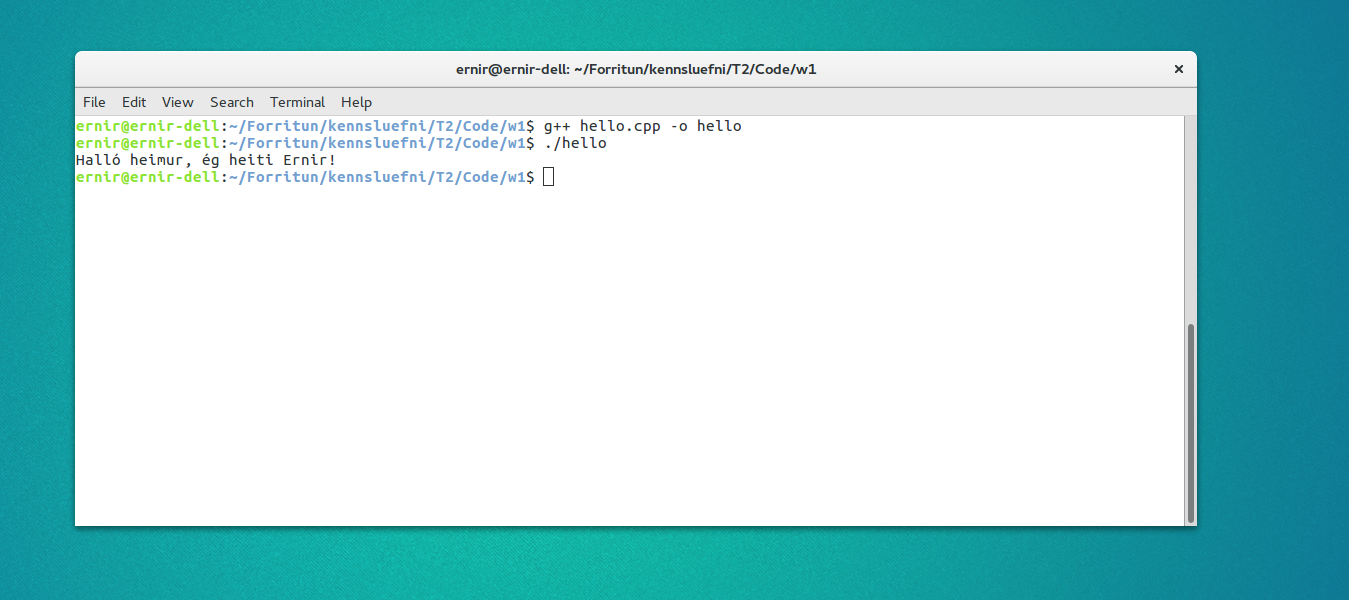
\includegraphics[width=\textwidth]{hello-ernir}
\end{center}


\section{Spurning 2}
Þetta er \href{https://projecteuler.net/problem=9}{Project Euler verkefni 9}.

Látum Pýþagóríska þrennd vera þrennd jákvæðra heiltalna $a,b,c$ svo að $a < b < c$ og $a^2 + b^2 = c^2$. Til dæmis er $3,4,5$ Pýþagórísk þrennd því að $3^2 + 4^2 = 5^2$.

Til er nákvæmlega ein Pýþagórísk þrennd þar sem $a + b + c = 1000$.\footnote{Uppfærsla: Talan hefur verið lagfærð, hér stóð áður 100.}

Skrifið C++ fall sem finnur þessa Pýþagórísku þrennd og skilar margfeldinu $abc$.

\newpage

\section{Spurning 3}
Þetta er \href{https://projecteuler.net/problem=46}{Project Euler verkefni 46}.

Christian nokkur Goldbach setti fram ýmsar tilgátur. Ein þeirra var að sérhverja samsetta oddatölu mætti skrifa sem summu prímtölu $p$ og tvöfaldri heiltölu í öðru veldi.

\begin{align*}
9 &= 7 + 2\cdot1^2\\
15 &= 7 + 2\cdot2^2\\
21 &= 3 + 2\cdot3^2\\
25 &= 7 + 2\cdot3^2\\
27 &= 19 + 2\cdot2^2\\
33 &= 31 + 2\cdot1^2\\
\end{align*}


Þessi tiltekna tilgáta reyndist hins vegar vera röng.

Skrifið C++ fall sem skilar þeirri samsettu oddatölu sem er lægsta mótdæmið gegn þessari tilgátu Goldbachs.

\paragraph{Ábending:} Mótdæmi undir 10000 er til.

\section{Spurning 4}
Þetta er \href{https://projecteuler.net/problem=14}{Project Euler verkefni 14}.

Collatz-runa er skilgreind fyrir allar jákvæðar heiltölur $n$ á eftirfarandi hátt:

Ef $n$ er slétt tala er næsta tala í rununni $n/2$. Ef $n$ er oddatala er næsta tala í rununni $3n +1$.

Þannig gefur upphafstalan $13$ Collatz-rununa $13 \to 40 \to 20 \to 10 \to 5 \to 16 \to 8 \to 4 \to 2 \to 1$, sem endar á $1$ og er af lengd 10. Talið er að allar runur skilgreindar með þessum hætti endi á $1$, en það hefur ekki verið sannað.

Skrifið C++ fall sem tekur inn jákvæða heiltölu $m$ og skilar þeirri upphafstölu minni en $m$ sem gefur lengstu Collatz-rununa.

Hvaða upphafstala minni en milljón gefur lengstu Collatz-rununa? Skilið tölunni og fallinu.

\paragraph{Ábendingar:} Óskilvirk forrit geta ekki leyst vandamálið fyrir ``stórar'' tölur á skynsamlegum tíma.

Sú upphafstala minni en 10 sem gefur lengstu rununa er 9. Sú upphafstala minni en 100 er 97. Sú upphafstala minni en 1000 sem gefur lengstu rununa er 871.

\vfill

\includegraphics[width=0.5\linewidth]{hi-von-logo}
\end{document}